
%%%%%%%%%%%%%%%%%%%%%%%%%%
\chapter{Introduction}
\label{ch:1Introduction}

Seizures are ephemeral states of irregular brain function. They are associated with temporary loss of consciousness and physical motor control. It is accepted by the epilepsy community that predicting future seizures a few minutes or more before occurring is a worthy goal \cite{kelley2009ninds, dumanis2017seizure}.

This thesis lays forth an exploration of existing approaches with new, noninvasive EEG datasets, as well as the development of a probabilistic computational model for unsupervised, or weakly supervised, seizure detection and prediction.

\section{Background}
Here we review common literature related to epilepsy prediction from EEG data, as well as probabilistic modeling, machine learning and Bayesian inference.

\subsection{Epileptic seizures}
Epilepsy is broadly defined by recurring unprovoked seizures. Epilepsy is characterized by hyper-synchronous activity spreading in the brain. In some individuals, this pathology can vary with time; seizures can form in a nonepileptic brain, show evolving dynamics, and even be resolved, allowing some patients seizure-freedom \cite{kandel2000principles}.

A complete understanding of epilepsy requires accounting for the high variability in symptoms across patients, as depicted by the many classes of epilepsy reported in the literature. The taxonomy of epilepsy involves groups of seizure types, epilepsy types, behavioural symptoms and recognizable etiologies (see Figure I. in \cite{scheffer2017ilae}).

\subsection{EEGs: electric potential recordings}
Electroencephalography (EEG) is a primary modality in the study of epilepsy (see figure \ref{fig:c1intro:eeg}). By capturing smoothed aggregations of local-field-potentials across cortical neural populations, the EEG is effective in capturing real-time neural firing dynamics. In particular, multiple channels measuring simultaneous activity across the scalp allow complex analyses of nonlinear spatiotemporal correlation from different brain regions.

EEGs may be intracranial (iEEG) or placed on the scalp's surface (sEEG). iEEG has a higher signal-to-noise ratio, but sEEG has the advantage of noninvasiveness. In any case, the resulting data has the form of a high-frequency multivariable time-series.

\begin{figure}[h]
    \centering
    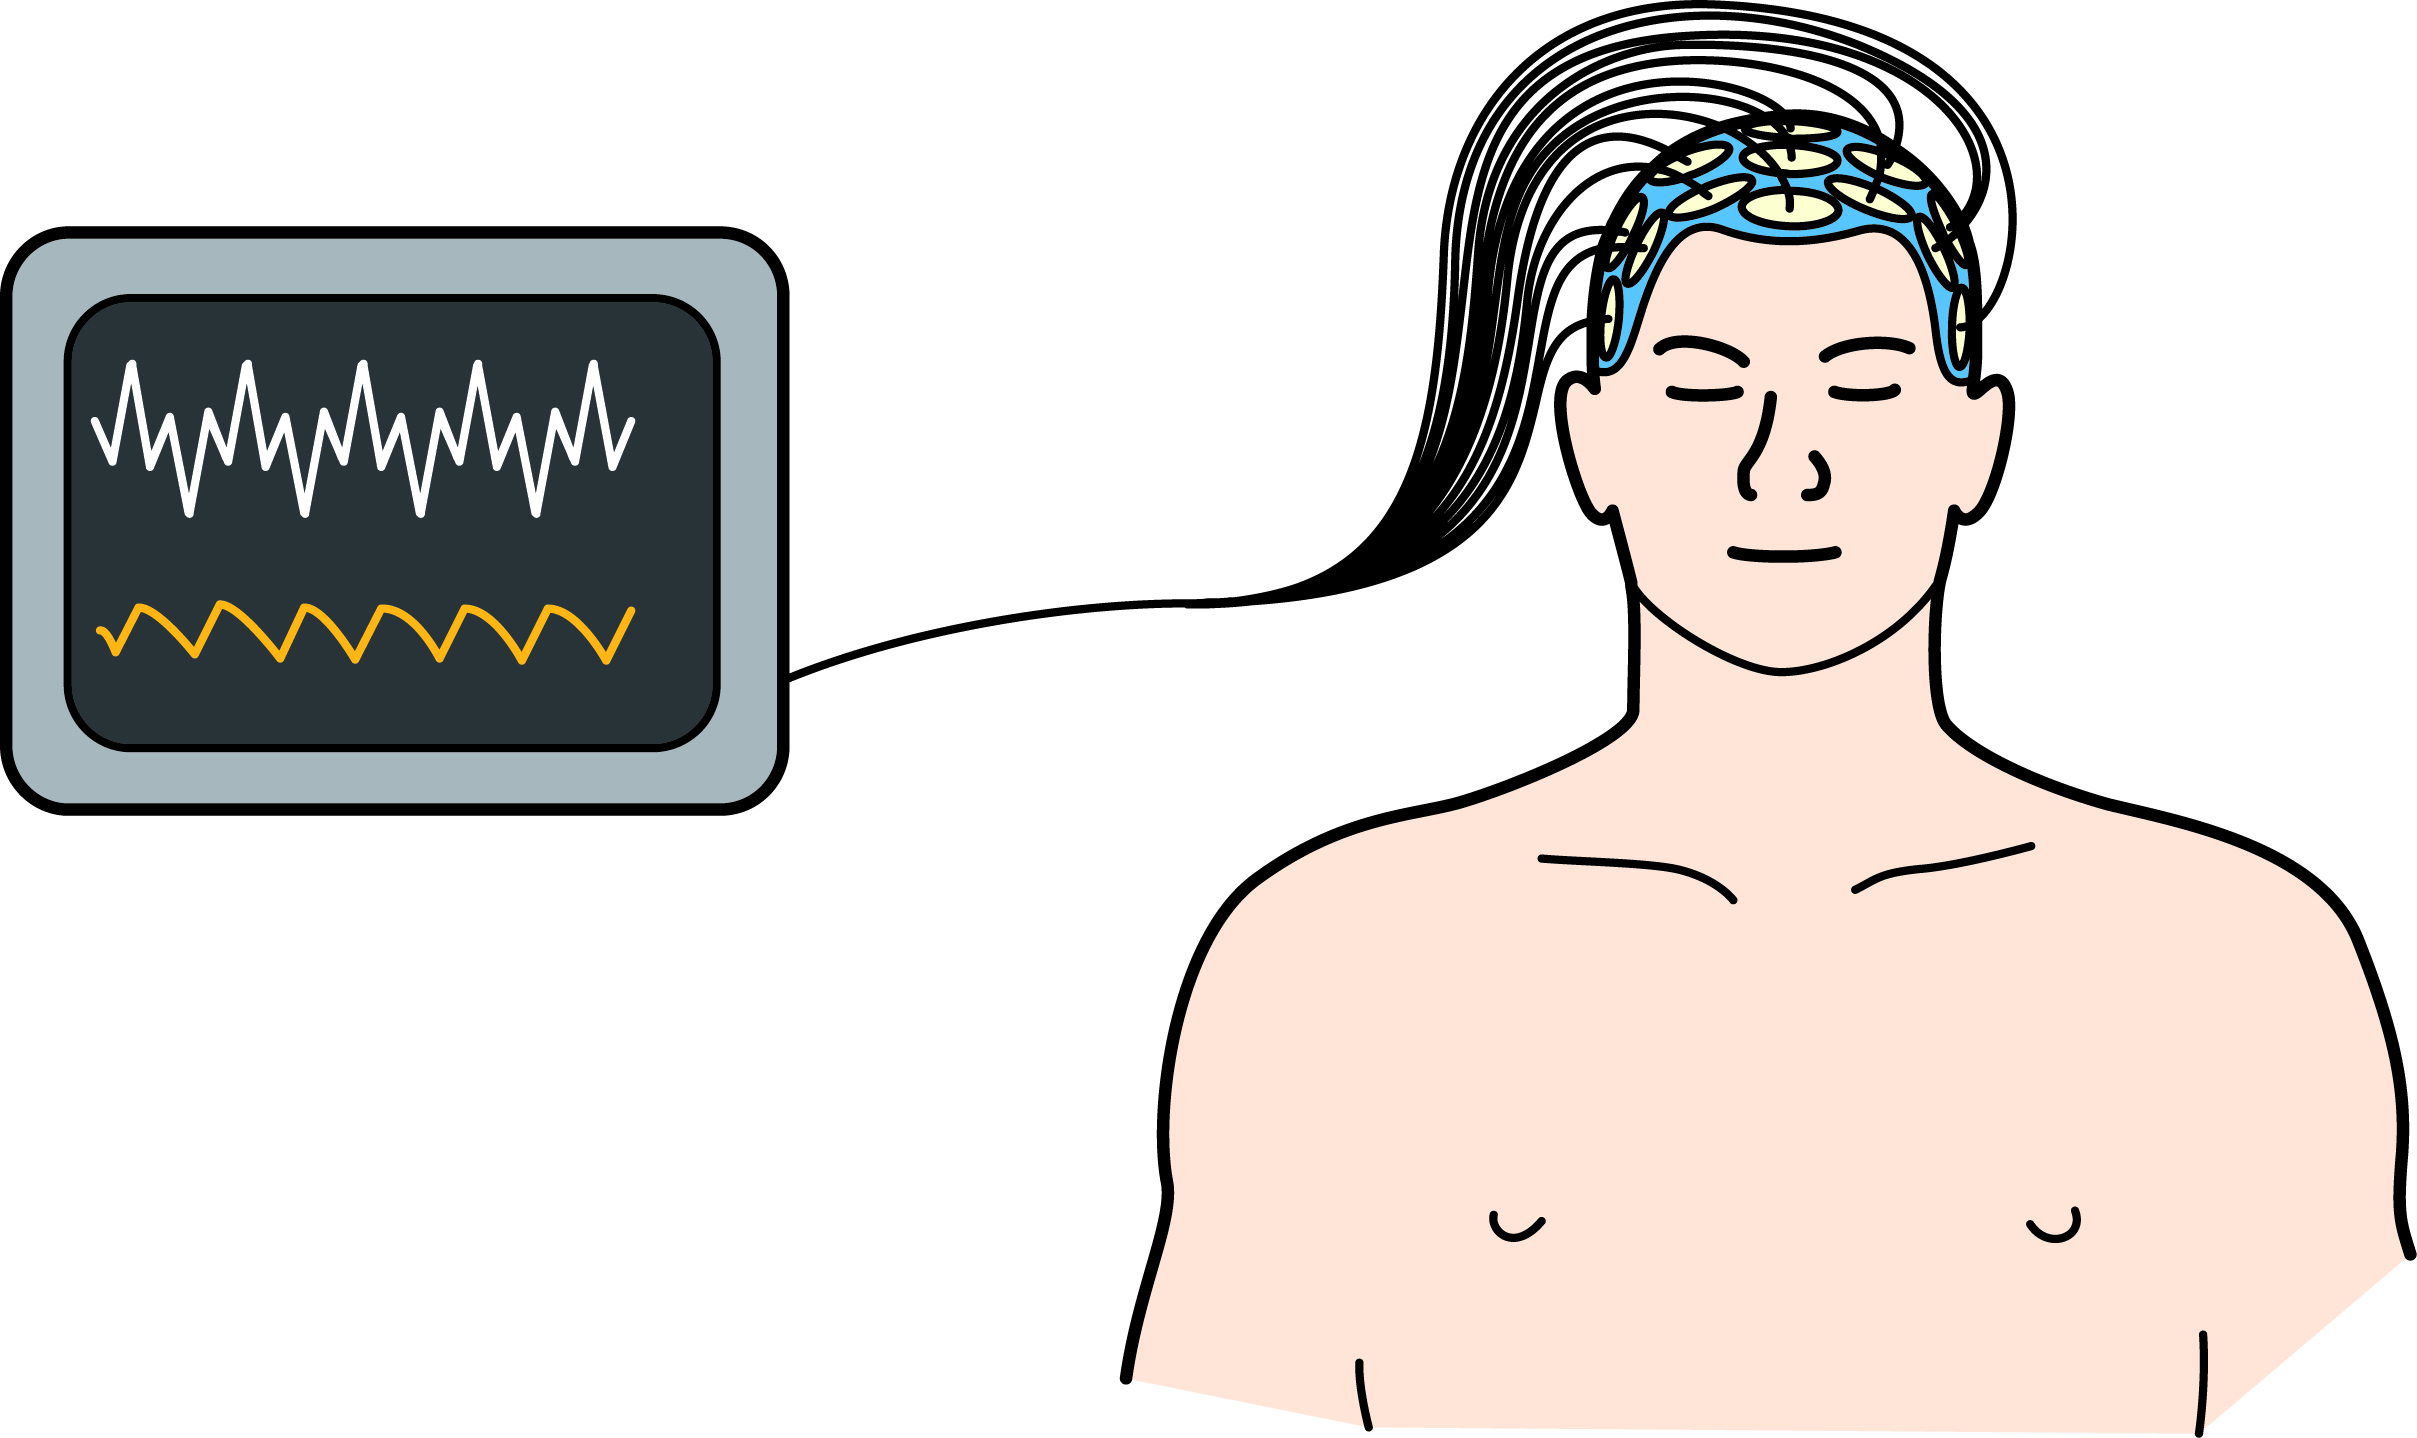
\includegraphics[width=\textwidth]{c1Introduction/eeg_easy_pics.jpg}
    \Caption{Electroencephalography (EEG) art}{\\\href{https://www.flickr.com/photos/easy-pics/9408344706}{eeg} from The Clear Communication People, licensed under \href{https://creativecommons.org/licenses/by-nc-nd/2.0/}{CC BY-NC-ND 2.0}.\\
    EEG is a form of neuroimagery with high temporal accuracy. In the noninvasive setup, a wearable cap holds electrodes in contact with the scalp. The electric potentials induced by the brain are transmitted to a digital recording system for data analysis.}
    \label{fig:c1intro:eeg}
\end{figure}

% The terms local field potentials (LFPs), electrocorticography\footnote{also termed intracranial EEG.} (ECoG) and electroencephalography (EEG) all commonly refer to measurements of electric potential: either in nerve tissue, on the directly exposed surface of the brain, or on the surface of the scalp, respectively. These types of recording apparatuses measure the summed electric activity of populations of individual cells (e.g., neurons).

For seizure monitoring and epilepsy diagnosis, video-electroencephalograms (vEEG) are the standard systems used in clinical settings. The vEEG records simultaneously videography and EEG from a particular subject, so that clinicians can observe both visual and electrophysiological epilepsy-related phenomena. EEG is also used for patient evaluation during outpatients visits, and in the ICU these sessions typically do not include video monitoring. In such cases, documentation of seizures is a challenging task which can be alleviated with seizure detection algorithms \cite{goldstein2021documentation}.

\subsection{Detecting and predicting seizures}
Computational seizure detection and forecasting with EEG data continues to be an active field of research since the 1970's \cite{mormann2007seizure, kuhlmann2018seizure}. Nonlinear methods were used in the 90's for analyzing cyclical, clustering and other time dependencies of seizure occurrences \cite{iasemidis1994time}. In the first decade of the millenium, models of EEG signals were developed to harness the dynamical processes involved in seizure generation for seizure forecasting \cite{kalitzin2005electrical}. Pattern recognition, including deep learning classifiers, have been shown to provide above chance classification in more than half of reported subjects \cite{mirowski2008comparing,mormann2016seizure}. The last two decades have seen unprecedented efforts from physicians, computer scientists and engineers to develop detective and predictive systems for epilepsy seizures \cite{jirsa2017virtual,nejedly2019deep, maimaiti2021overview}.

\subsection{Probabilistic modeling of seizure risk in epilepsy}
The global clustering and cyclical properties of epilepsy seizures has led researchers to use probabilistic models for seizure risk estimation.
% Probabilistic programming languages, which ease the Bayesian inference of complex models, have been applied to understanding seizure generation and propagation \cite{vattikonda2021identifying}.
\citet{craley2019integrating} implement a hybrid deep-learning and probabilistic-graphical-model approach and show that it outperforms baseline methods at seizure detection. A logistic regression model, tweaked with Bayes' rule to incorporate a subject-specific prior, was shown to improve forecasting in humans \cite{karoly2017circadian}. Stochastic point process models have shown promising results for integrating prior information with real-time likelihood assessments to produce forecasts of seizures hours to days in advance, although prospective clinical studies are still required to validate the applicability of these algorithms \cite{proix2021forecasting}.

\subsection{Supervised machine learning and the data labeling problem}
Prior work on automated seizure detection and prediction has focused on training machine learning models to classify EEG segments labeled as ictal, preictal or interictal. This requires expert labeling of EEG datasets for seizure events, which is both time consuming and requires extensive training. The dependence of supervised machine learning classifiers on expert-level domain knowledge makes these algorithms unsuitable for real-world forecasting devices, since expert categorical labeling solutions are still not available at scale \cite{rasheed2020machine}.
Furthermore, even clinical-grade annotations, considered to be the "gold standard" in seizure documentation, suffer from judgement bias \cite{halford2015inter}.

